%!TEX program = xelatex
% run this file: xelatex -shell-escape slides.tex
\documentclass{beamer}

\usepackage{blindtext}
\usepackage{minted}
\usepackage{tcolorbox}
\usepackage{etoolbox}
\BeforeBeginEnvironment{minted}{\begin{tcolorbox}}%
\AfterEndEnvironment{minted}{\end{tcolorbox}}%

\usetheme{Execushares}

% define title and subtitle here
\title{Introduction to C and Unix}
\subtitle{CS537 Section 304}

\author{Kevin Bao, Cheng Su}
\date{\today}

\begin{document}
	\setcounter{framenumber}{0}
	\frame{\titlepage}
	\setcounter{showProgressBar}{1}
	\setcounter{showSlideNumbers}{1}

	% define contents here
	\begin{frame}
		\frametitle{Contents}
		\begin{enumerate}
			\item Overview \\
			\item Introduction to C \\ 
				\textcolor{ExecusharesGrey}{\footnotesize\hspace{1em} pointer and man}
			\item Introduction to Unix  \\ 
				\textcolor{ExecusharesGrey}{\footnotesize\hspace{1em} shell, ssh, gcc, make and vi}
			\item Suggested Readings \\ 
				\textcolor{ExecusharesGrey}{\footnotesize\hspace{1em} books and blogs}
		\end{enumerate}
	\end{frame}

	% define each slides here
	% 1.overview
  \begin{frame}
    \frametitle{Overview}
		\begin{enumerate}
			\item 5 projects
			\item Use C
			\item Vedios are useful
			\item Start early
			\item Mind your code quality
		\end{enumerate}
	\end{frame}

	% 1.pointer
  \begin{frame}
    \frametitle{What is a pointer}
    \begin{enumerate}
      \item For now, treat the memory as a giant array
      \item Pointer is like an index
      \item How can we know the size of the data?
    \end{enumerate}
  \end{frame}

	% 2.man
  \begin{frame}
    \frametitle{Man}
    \begin{enumerate}
      \item man man
      \item An interface to the on-line reference manuals
      \item We will mainly use man 2 and man 3
    \end{enumerate}
  \end{frame}

	% 3.open terminal
  \begin{frame}
    \frametitle{Open your terminal}
    \begin{enumerate}
      \item Linux: Ctrl-Alt-T
      \item Mac OS: Cmd-Space, search ``terminal''
      \item Windows: Get a computer with 1 or 2
    \end{enumerate}
  \end{frame}

	% 4.download code
	\begin{frame}[fragile]
		\frametitle{Download our github repo}
		https://github.com/c21/UWOS
		\begin{center}		
		\begin{minted}{bash}
			$ git clone https://github.com/c21/UWOS.git
			$ cd UWOS/1-intro/demo/c
			$ ls
			pointer0.c  pointer1.c  pointer2.c ...
			$ cat pointer0.c
    \end{minted}
		\end{center}
	\end{frame}

	% 2.shell
	\begin{frame}
		\frametitle{Shell: a servant}
		You write command, shell runs it for you.
		\begin{center}
		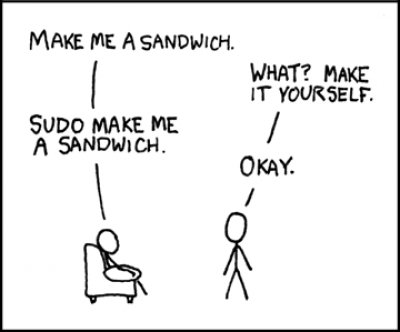
\includegraphics[width=0.6\textwidth, height=0.6\textheight]{img/sudo.jpg}
		\end{center}
	\end{frame}

	% 2.shell - command
	\begin{frame}[fragile]
		\frametitle{A philosophical shell}
		Who am I ...
		\begin{center}
		\begin{minted}{bash}
			$ whoami
			chengsu

			$ date
			Sat Sep  3 20:57:13 CDT 2016

			$ pwd
			/home/chengsu 
		\end{minted}
		\end{center}	
	\end{frame}

	% 3.ssh
	\begin{frame}[fragile]
		\frametitle{SSH}
		Login to a remote computer.
		\begin{center}
		\begin{minted}{bash}
			$ ssh remote_username@remote_host
			$ run-any-command-on-remote-computer
			$ logout
    \end{minted}
		\end{center}
		\begin{itemize}
      \item Options: -X, etc.
			\begin{itemize}
        \item open a game in /usr/games
      \end{itemize}
			\item No hassle of password? \\
			\begin{itemize}
				\item ssh keys
				\item sshpass
			\end{itemize}	
		\end{itemize}
	\end{frame}

	% 3-2.ssh code
	\begin{frame}[fragile]
		\frametitle{Try SSH yourself}
		Open a sudoku game on lab's computer
		\begin{center}
		\begin{minted}{bash}
			$ ssh -X your-cs-name@emperor-01.cs.wisc.edu
			$ cd /usr/games/
			$ ls
			$ ./gnome-sudoku
			$ logout
		\end{minted}
		\end{center}
	\end{frame}

	% 4.gcc
  \begin{frame}
    \frametitle{GCC}
    GNU Compiler Collection.

		\begin{enumerate}
      \item \textbf{\textit{preprocessing}} (C code) 
      \item compilation (assembly code)
			\item assembly (binary code)
			\item linking (executable binary code)
    \end{enumerate}
	\end{frame}

	% 4-2.gcc code
	\begin{frame}[fragile]
		\frametitle{Try preprocessing yourself}
		Preprocess test.c
		\begin{center}
		\begin{minted}{bash}
			$ cd ~/UWOS/1-intro/demo/unix
			$ ls
			Makefile  test.c  test.h
			$ cat test.h
			$ cat test.c
			$ gcc -E test.c >prep_test.c
			$ cat prep_test.c
		\end{minted}
		\end{center}
	\end{frame}


	% 5.make
  \begin{frame}[fragile]
    \frametitle{Make}
    Recipe to cook (build) programs. 
    \begin{minted}{make}
			target: prerequisite1 prerequisite2 ...
			    command1
			    command2
			    ...
    \end{minted}
		\begin{itemize}
      \item Efficiency (compare timestamps of \textit{target} and \textit{prereqs})
			\begin{itemize}
        \item make ; make
      \end{itemize}
			\item Other usage (not serious)
			\begin{itemize}
        \item workflow control: \textcolor{ExecusharesGrey}{\footnotesize\hspace{1em}\url{http://widgetsandshit.com/teddziuba/2011/02/stupid-unix-tricks-workflow-control-with-gnu-make.html}}
      \end{itemize}						 
    \end{itemize}	
	\end{frame}

	% 6.vi
	\begin{frame}
		\frametitle{Vi: text editor}
		
		\begin{itemize}
			\item \small Basic usage
			\begin{itemize}
				\item \small write code: i (insert mode)
				\item \small write command: <Esc> (command mode)
				\item \small go to a line: :12 (go to 12th line)
				\item \small copy a line: yy
				\item \small paste a line: p
				\item \small search a word: /dog (search word: dog)
				\item \small undo: u
			\end{itemize} 
      \item \small How to learn Vi/Vim
      \begin{itemize}
        \item \small vimtutor
				\item \small \url{http://www.openvim.com}
				\item \small even a game to play: \url{http://vim-adventures.com}
      \end{itemize}
      \item \small Configure Vi
      \begin{itemize}
				\item \small dotfile: .vimrc (set indentation to 2 space)
			\end{itemize}
    \end{itemize}
  \end{frame}

	% suggested readings
	\begin{frame}
    \frametitle{Suggested Readings}
		\begin{itemize}
        \item \small C
        \begin{itemize}
          \item \small \href{https://www.amazon.com/Programming-Language-Prentice-Hall-Software/dp/0131103628}{The C Programming Language (Chapter 5, 8.7)}
          \item \small \href{https://www.amazon.com/Expert-Programming-Peter-van-Linden/dp/0131774298}{Expert C Programming: Deep C Secrets (Chapter 1)}
        \end{itemize}
    \end{itemize}

		\begin{itemize}
        \item \small Unix (Basic) 
				\begin{itemize}
					\item \small \href{http://matt.might.net/articles/basic-unix}{Survival guide for Unix newbies}
					\item \small \href{http://matt.might.net/articles/settling-into-unix}{Settling into Unix}
					\item \small \href{https://www.amazon.com/Unix-Programming-Environment-Prentice-Hall-Software/dp/013937681X}{The Unix Programming Environment (Chapter 1)}
			\end{itemize}	
		\end{itemize}

		\begin{itemize}
        \item \small GCC, GDB and Make
        \begin{itemize}
          \item \small \href{http://pages.cs.wisc.edu/~remzi/OSTEP/lab-tutorial.pdf}{CS537 Lab Tutorial}
        \end{itemize}
    \end{itemize}
	
		\begin{itemize}
        \item \small Our Material
        \begin{itemize}
          \item \small \url{https://github.com/c21/UWOS}
        \end{itemize}
    \end{itemize}
	\end{frame}	

\end{document}
